\exo

La fonction $g$ est définie sur l'intervalle $[-3~;~5]$ par la courbe ci-dessous.

\begin{center}
\newrgbcolor{wqwqwq}{0.3764705882352941 0.3764705882352941 0.3764705882352941}
\psset{xunit=1cm,yunit=1cm,algebraic=true,dimen=middle,dotstyle=o,dotsize=5pt 0,linewidth=1.6pt,arrowsize=3pt 2,arrowinset=0.25}
\begin{pspicture*}(-4.5,-2.5)(6.5,2.5)
\multips(0,-7)(0,1){15}{\psline[linestyle=dashed,linecap=1,dash=1.5pt 1.5pt,linewidth=0.4pt,linecolor=wqwqwq]{c-c}(-4.5,0)(6.5,0)}
\multips(-11,0)(1,0){23}{\psline[linestyle=dashed,linecap=1,dash=1.5pt 1.5pt,linewidth=0.4pt,linecolor=wqwqwq]{c-c}(0,-2.5)(0,2.5)}
\psaxes[labelFontSize=\scriptstyle,xAxis=true,yAxis=true,Dx=1,Dy=1,ticksize=-2pt 0,subticks=2]{->}(0,0)(-4.5,-2.5)(6.5,2.5)
\psline[linewidth=2pt](-3,1)(0,-2)
\psline[linewidth=2pt](0,-2)(2,2)
\psline[linewidth=2pt](2,2)(5,-1)
\begin{scriptsize}
\psdots[dotstyle=+](-3,1)
\psdots[dotstyle=+](5,-1)
\end{scriptsize}
\end{pspicture*}
\end{center}

Donner un encadrement de $g(x)$ le plus précis possible sur chacun des intervalles suivants.


a)~ $[-3~;~5]$ \hspace{0.8cm} b)~$[-3~;~1]$ \hspace{0.8cm} c)~$[1~;~5]$ \hspace{0.8cm} d)~$[-1~;~3]$ 



\exo \textit{[Raisonner, représenter]}

Le graphique ci-dessous donne la courbe $C_f$ représentative de la fonction $f$ : 
\begin{center}\small

\psset{unit=0.8cm}
\begin{pspicture*}(-6.5,-3.9)(7.6,3.9)
\psgrid[subgriddiv=0,gridlabels=0,gridcolor=lightgray](0,0)(-6.5,-3.9)(7.6,3.9)
\psset{algebraic=true,dotstyle=o,dotsize=3pt 0,linewidth=1pt,arrowsize=3pt 2,arrowinset=0.25}
\psaxes[labelFontSize=\scriptstyle,xAxis=true,yAxis=true,Dx=1,Dy=1,ticksize=-2pt 0,subticks=2]{->}(0,0)(-6.5,-3.9)(7.6,3.9)
\psdots[dotstyle=*](-6,3)(7,0)
\pscurve[linewidth=2pt]{-}(-6,3)(-5,1)(-4,0)(-3,-1)(-1,0)(0,1)(2,2)(3,1)(4,0)(5,-1)(7,0)
\rput{0}(-5.5,3.2){\textbf{$C_f$}}
\end{pspicture*}

\end{center}

\begin{enumerate}
\item Donner l’ensemble de définition I de la fonction $f$.
\item Compléter le tableau de valeurs suivant:

\begin{center}
\begin{tabular}{|*{6}{p{1cm}|}}
\hline
\centering $x$ &  \centering$-4$ &  &\centering$-1$ & \centering $0$ & \centering$1$ \tabularnewline
\hline
\centering $f(x)$ & & \centering $-1$ & & & \tabularnewline
\hline
\end{tabular}
\end{center}
\item Utiliser ces résultats pour prouver que la fonction $f$ n'est ni paire ni impaire.  
\item Déterminer les extremums de $f(x)$ sur I.
\item Résoudre l'équation $f(x)=1$ en justifiant.
\item Résoudre graphiquement l’inéquation : $f(x) > 1$.
\item Donner les solutions de l'inéquation : $f(x) < 0$.
\end{enumerate}



\exo \textit{[Chercher, communiquer]}

On a tracé ci-dessous dans un repère la courbe représentative d'une fonction $f$.
\begin{center}\small

\psset{unit=0.8cm}
\begin{pspicture*}(-6.3,-4.3)(3.3,3.3)
\psgrid[subgriddiv=0,gridlabels=0,gridcolor=lightgray](0,0)(-6.3,-4.3)(3.3,3.3)
\psset{algebraic=true,dotstyle=o,dotsize=3pt 0,linewidth=1pt,arrowsize=3pt 2,arrowinset=0.25}
\psaxes[labelFontSize=\scriptstyle,xAxis=true,yAxis=true,Dx=1,Dy=1,ticksize=-2pt 0,subticks=2]{->}(0,0)(-6.3,-4.3)(3.3,3.3)
\psdots[dotstyle=*](-6,2)(3,3)
\pscurve[linewidth=2pt]{-}(-6,2)(-4,0)(-2.5,-3)(-1,-4)(0.5,-3)(1.5,0)(3,3)
\rput{0}(-5.5,2.2){\textbf{$C_f$}}
\end{pspicture*}

\end{center}
\begin{enumerate}[label=\arabic*.]
\item Donner l’ensemble de définition I de la fonction $f$.
\item Déterminer $f(-1)$ et $f(-3)$.
\item Encadrer $f(x)$ sur I.
\item En expliquant la méthode, résoudre graphiquement l'équation: $f(x)=0$.
\item En expliquant la méthode, résoudre graphiquement l'inéquation: $f(x)\leqslant-3$.
\end{enumerate}

\exo \textit{[Représenter]}
\begin{enumerate}
\item Dresser le tableau de signes de la fonction $f$ représentée dans l'exercice 1 p 80 du cahier d'exercices.
\item Dresser le tableau de signes de la fonction $f$ représentée dans l'exercice 1 de cette fiche.
\item  Dans un repère, tracer une courbe représentative d'une fonction $f$ dont le tableau de signes est le suivant:

\begin{center}
\begin{tikzpicture}
\tkzTabInit[espcl=1.5]%
{$x$ / 1,$f(x)$ / 1}%
{$-7$,$-3$,$1$,$2$,$4$}%
\tkzTabLine{,+,z,-,z,-,z,+,}
\end{tikzpicture}
\end{center}

\end{enumerate}

\exo \textit{[Raisonner,représenter, communiquer]}

Dans un repère, $\mathcal{C}_f$ et $\mathcal{C}_g$ sont les courbes représentatives de fonctions $f$ et $g$ définies sur $[-3 ;3]$.

\bigskip


\begin{minipage}{0.6\linewidth}
\begin{enumerate}[label=\arabic*.]
\item Indiquer le minimum et le maximum de $g$ sur $[-3 ;3]$ et préciser la valeur de $x$ pour laquelle il est atteint. 
\item Dresser le tableau de signe de la fonction $g$. 
\item Résoudre l'équation $f(x)=g(x)$ en justifiant.
\item Résoudre l'inéquation $f(x)>g(x)$ en justifiant.
\item Résoudre l'inéquation $f(x) \leqslant g(x)$
\end{enumerate}
\end{minipage}
\hfill
\begin{minipage}{0.4\linewidth}
\begin{center}
\psset{xunit=0.62cm,yunit=0.62cm,arrowsize=2pt 2}
\begin{pspicture}(-3.4,-2.3)(3.4,3.3)
  \psgrid[subgriddiv=1,gridlabels=0pt,gridcolor=cyan!25](-3,-2)(3,3)
  \psaxes[labels=none,ticks=none]{->}(0,0)(-3.3,-2.2)(3.3,3.2)
  \rput(-0.35,-0.35){O}
  \rput(-3,-0.35){$-3$}\rput(1,-0.35){$1$}\rput(3,-0.35){$3$}
  \rput(-0.35,1){$1$}\rput(-0.35,2){$2$}
  \psline[linecolor=green!65!black,linewidth=1.4pt](-3,-2)(1,1)(3,2.5)
  \pscurve[linecolor=blue,linewidth=1.6pt](-3,2)(-2,-1)(-1,-2)(0,-2)(1,1)(2,2.4)(3,3)
  \psdots[dotsize=4pt,linecolor=blue](-3,2)(-2,-1)(0,-2)(1,1)(3,3)
  \rput(-2.55,1.25){\blue $\mathcal C_f$}
  \rput(2.65,2.05){\green $\mathcal C_g$}
\end{pspicture}
\end{center}
\end{minipage}




\exo \textit{[Chercher, Représenter]}

On considère les fonctions $f$ et $g$ dont la représentation graphique est donnée ci-dessous.

\begin{center}\small

\psset{unit=0.8cm}
\begin{pspicture*}(-6.2,-4.3)(3.6,4.6)
\psgrid[subgriddiv=0,gridlabels=0,gridcolor=lightgray](0,0)(-6.2,-4.3)(3.6,4.6)
\psset{algebraic=true,dotstyle=o,dotsize=3pt 0,linewidth=1pt,arrowsize=3pt 2,arrowinset=0.25}
\psaxes[labelFontSize=\scriptstyle,xAxis=true,yAxis=true,Dx=1,Dy=1,ticksize=-2pt 0,subticks=2]{->}(0,0)(-6.2,-4.3)(3.6,4.6)
\psdots[dotstyle=*](-5.5,2)(2,2)(-5.5,-3)(2,-1.5)
\pscurve[linecolor=red, linewidth=2pt]{-}(-5.5,2)(-4,3.5)(-2.5,1)(-2,0)(-1,-2)(0,0)(0.5,1)(1,1.5)(2,2)
\rput{0}(-5.5,3){\textbf{$C_f$}}
\pscurve[linestyle=dashed,linecolor=blue,linewidth=2pt]{-}(-5.5,-3)(-3,0)(-2.5,1)(-1,2)(0,1.5)(0.5,1)(1,0.5)(2,-1.5)
\rput{0}(-5,-3.5){\textbf{$C_g$}}
\end{pspicture*}

\end{center}

\begin{enumerate}[label=\arabic*.]
\item Donner l’ensemble de définition I de ces deux fonctions.
\item Encadrer $f(x)$ sur I.
\item Dresser le tableau de signe de la fonction $f$. 
\item Résoudre graphiquement l’équation : $f(x) = g(x)$.
\item Résoudre graphiquement l’inéquation :$f(x) \leqslant g(x)$. 
\end{enumerate}





